\documentclass[tikz,border=6pt]{standalone}
% =============================================================================
%  PREAMBULE COMMUN DES SCHEMAS DU SUPPORT DE SOUTENANCE (ENSAE, octobre 2026)
%
%  Les schemas sont des VISUELS DE DIAPOSITIVE, pas des figures de donnees : ils
%  prennent donc la palette du gabarit de presentation Nexialog, recopiee de
%  build_soutenance_ppt.py, et jamais celle de style_nexialog.py, qui reste la
%  source unique des couleurs des figures du memoire.
%
%  AUCUN NOMBRE DE RESULTAT N'Y FIGURE. Un nombre dessine dans une image echappe
%  au controle du support, qui verifie chaque nombre de texte contre le rapport.
%  Les schemas portent des symboles et des equations, recopiees du rapport.
%
%  Polices : Segoe UI pour le texte, comme le corps du gabarit ; Latin Modern Math
%  pour les formules, celle du rapport. Chaque schema se dessine A SA TAILLE FINALE
%  sur la diapositive, si bien qu'un corps de 14 pt ici vaut 14 pt a l'ecran.
% =============================================================================
\usepackage{fontspec}
\usepackage{unicode-math}
\setmainfont{Segoe UI}
\setsansfont{Segoe UI}
\setmathfont{latinmodern-math.otf}
\usetikzlibrary{positioning,arrows.meta,calc,fit,backgrounds,shapes.geometric,decorations.pathreplacing}

\definecolor{ardoise}{HTML}{223E55}   % titres et aplats du gabarit
\definecolor{profond}{HTML}{192E3F}
\definecolor{acier}{HTML}{435B6E}
\definecolor{encre}{HTML}{122738}     % texte courant
\definecolor{gris}{HTML}{595959}      % texte secondaire
\definecolor{accent}{HTML}{B10031}    % rouge de marque
\definecolor{clair}{HTML}{F2F2F2}
\definecolor{filet}{HTML}{D9D9D9}

\newcommand{\corps}{\fontsize{14}{17}\selectfont}
\newcommand{\petit}{\fontsize{12}{14.5}\selectfont}
\newcommand{\grand}{\fontsize{16}{19}\selectfont}
\tikzset{
  >={Stealth[length=7pt,width=6pt]},
  bloc/.style={draw=ardoise, line width=0.9pt, fill=white, rounded corners=3pt,
               inner sep=6pt, align=center, text=encre, font=\corps},
  bloc plein/.style={fill=ardoise, draw=ardoise, rounded corners=3pt, inner sep=6pt,
               align=center, text=white, font=\corps\bfseries},
  bloc accent/.style={fill=accent, draw=accent, rounded corners=3pt, inner sep=6pt,
               align=center, text=white, font=\corps\bfseries},
  fleche/.style={->, line width=1.3pt, draw=acier},
  fleche accent/.style={->, line width=1.6pt, draw=accent},
  legende/.style={font=\petit, text=gris, align=center},
}

% -----------------------------------------------------------------------------
%  Schema « le modele en un regard » (support de soutenance ENSAE), diapositive
%  qui precede les chapitres 4 a 6. Taille finale : 11,6 x 4,5 pouces.
%  Aucun nombre de resultat : seul « 99,5 % » figure, dans le quantile.
%  Formules et libelles recopies du rapport (chapitres_sfe/) :
%   - etat de conformite : 06_multietats.tex l. 34 (sans la valeur de gamma),
%     l. 39-41 (seuils K_bas, K_haut, dessines en axe), l. 19-20 (NC, PC, C)
%     et l. 31 (« Chaque pilier possede une capacite de conformite latente ») ;
%   - quatre canaux : 06_multietats.tex l. 72-87 ;
%   - frequence : 04_frequence_severite.tex l. 143-149 ; « nombre annuel N » :
%     09_resultats.tex l. 390 et note de synthese ;
%   - severite : 04_frequence_severite.tex l. 44-46 et 65 ;
%   - cascade : 05_cascade.tex l. 120 ; S_a : 05_cascade.tex l. 216-219 et
%     annexe_b_parametres_notations.tex l. 142 ;
%   - capital : 09_resultats.tex l. 386-391 (au secteur, m(A) n'apparait pas) ;
%     « perte d'un sinistre » : 10_robustesse.tex l. 292 ; « quantile de la
%     charge annuelle agregee » : 04_frequence_severite.tex l. 108 et
%     03_donnees.tex l. 252.
%  Les mots droits des formules (TRANS, max, VaR, bas, haut) sont composes dans
%  la fonte mathematique : sous unicode-math, \mathrm prendrait Segoe UI, d'ou sa
%  redefinition locale en \symup. TRANS et VaR gardent le \mathrm du rapport ;
%  bas et haut, en \text dans le rapport, sont ecrits en \symup pour la meme raison.
%  Disposition : chaque canal est aligne sur le bloc qu'il deplace, si bien que
%  toutes les fleches sont droites ou presque et qu'aucune ne croise un bloc.
% -----------------------------------------------------------------------------
\begin{document}
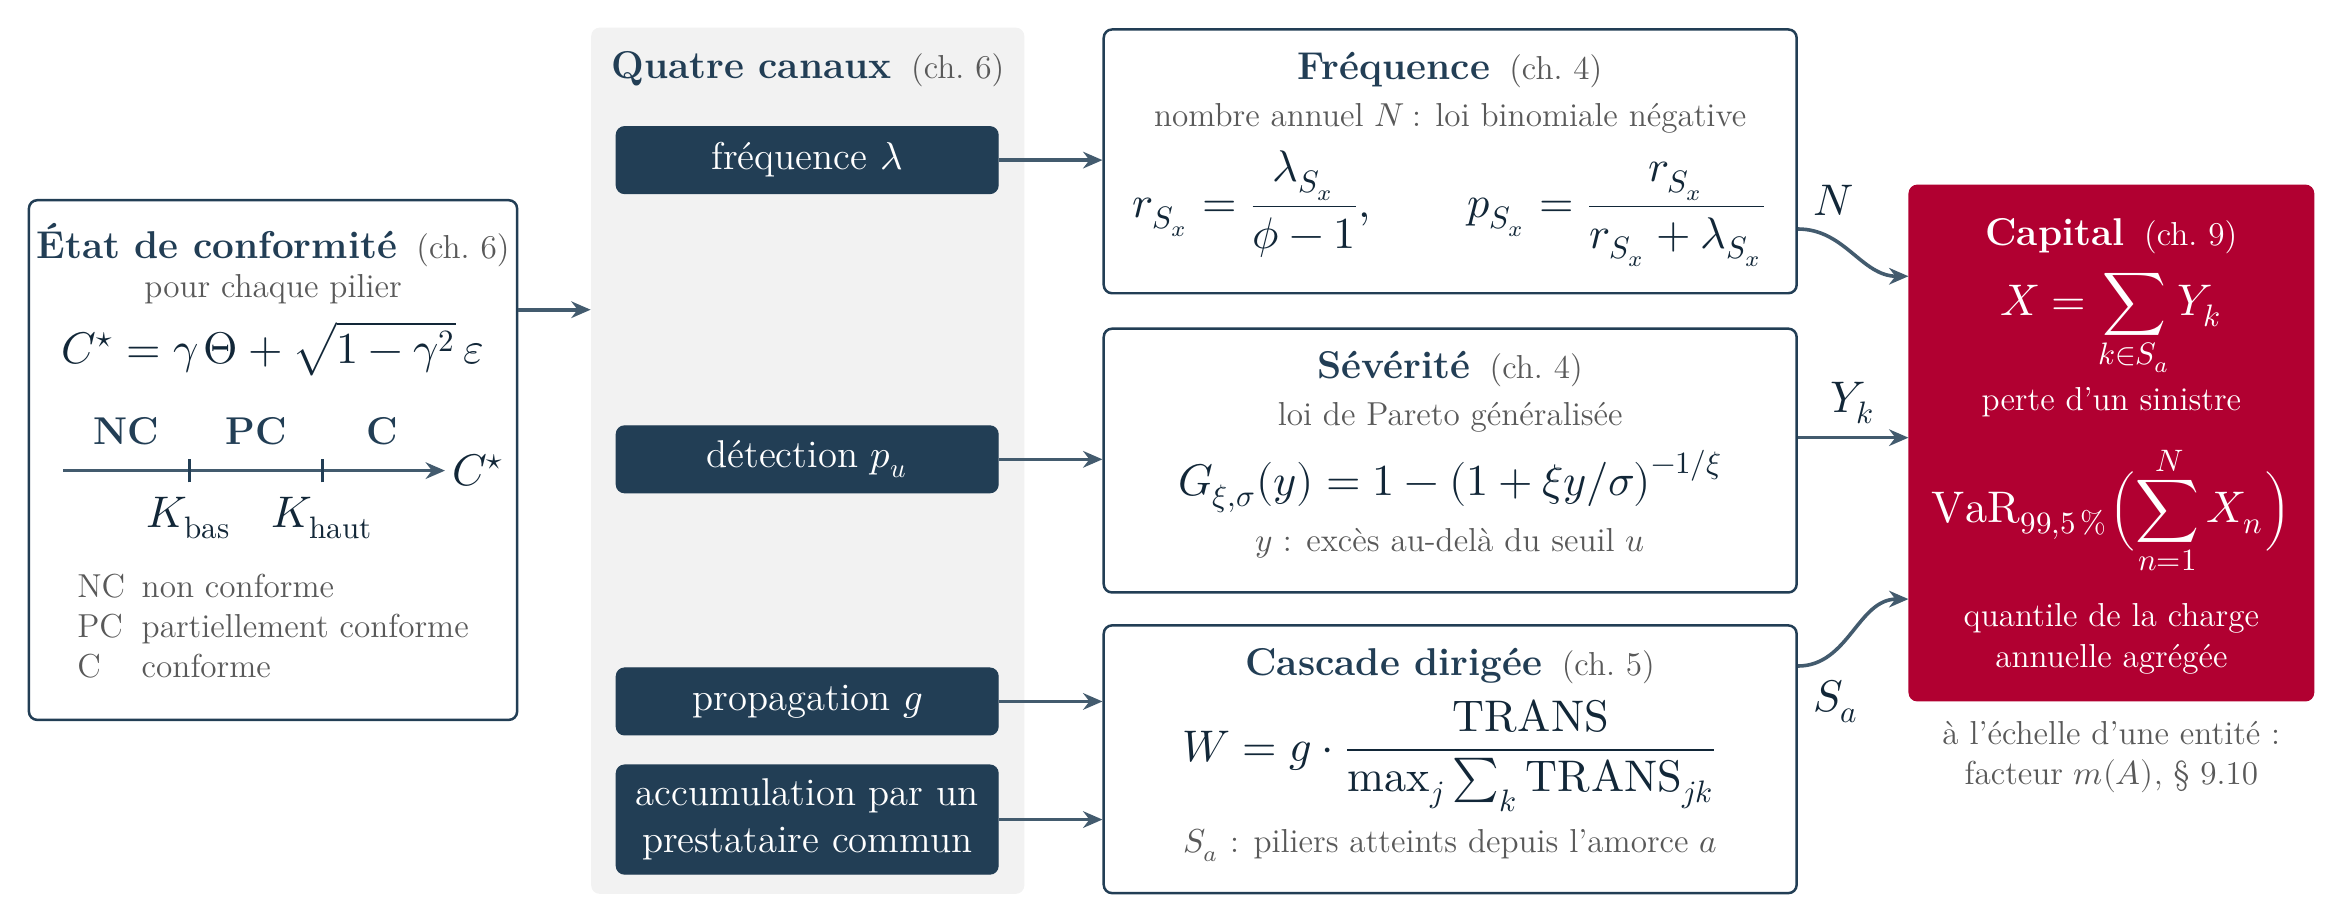
\begin{tikzpicture}[x=1cm, y=1cm,
  titre/.style={font=\corps\bfseries, text=ardoise, inner sep=0pt},
  formule/.style={font=\grand, text=encre, inner sep=0pt},
  texte/.style={font=\petit, text=gris, align=center, inner sep=0pt},
  pastille/.style={fill=ardoise, draw=ardoise, rounded corners=3pt, inner sep=5pt,
                   align=center, text=white, font=\corps, minimum width=4.85cm,
                   minimum height=0.85cm},
  etiquette/.style={font=\grand, text=encre, inner sep=2pt},
]
\newcommand{\chap}[1]{\enspace{\mdseries\petit\color{gris}(ch.~#1)}}
% mots droits des formules dans la fonte mathematique (voir l'en-tete)
\renewcommand{\mathrm}[1]{\symup{#1}}
\renewcommand{\max}{\mathop{\symup{max}}}

% cadre de la taille finale (la bordure de 6 pt s'ajoute autour)
\path (0,0) rectangle (29.04,11.0);

% ---- colonne 1 : etat de conformite (ch. 6) ---------------------------------
\node[bloc, minimum width=6.2cm, minimum height=6.6cm, anchor=south west] (etat) at (0,2.2) {};
\node[titre, anchor=north] at ([yshift=-0.3cm]etat.north) {État de conformité\chap{6}};
\node[texte, anchor=north] at ([yshift=-0.95cm]etat.north) {pour chaque pilier};
\node[formule, anchor=north] at ([yshift=-1.55cm]etat.north)
  {$C^\star = \gamma\,\Theta + \sqrt{1-\gamma^2}\,\varepsilon$};
\begin{scope}[shift={($(etat.north west)+(0.45,-3.45)$)}]
  \draw[->, line width=1.1pt, draw=acier] (0,0) -- (4.85,0)
    node[right, font=\grand, text=encre, inner sep=2pt] {$C^\star$};
  \foreach \x in {1.6,3.3} \draw[line width=1.1pt, draw=ardoise] (\x,-0.15) -- (\x,0.15);
  \node[font=\corps\bfseries, text=ardoise, anchor=south] at (0.8,0.2) {NC};
  \node[font=\corps\bfseries, text=ardoise, anchor=south] at (2.45,0.2) {PC};
  \node[font=\corps\bfseries, text=ardoise, anchor=south] at (4.05,0.2) {C};
  \node[font=\grand, text=encre, anchor=north] at (1.6,-0.22) {$K_{\symup{bas}}$};
  \node[font=\grand, text=encre, anchor=north] at (3.3,-0.22) {$K_{\symup{haut}}$};
\end{scope}
\node[texte, anchor=north] at ([yshift=-4.7cm]etat.north)
  {\begin{tabular}{@{}l@{\enspace}l@{}}NC & non conforme\\PC & partiellement conforme\\C & conforme\end{tabular}};

% ---- colonne 2 : quatre canaux (ch. 6) ----------------------------------------
\node[fill=clair, rounded corners=3pt, minimum width=5.5cm, minimum height=11.0cm,
      inner sep=0pt, anchor=south west] (canaux) at (7.15,0) {};
\node[titre, anchor=north] at ([yshift=-0.3cm]canaux.north) {Quatre canaux\chap{6}};
\node[pastille] (pF) at (9.9,9.325) {fréquence $\lambda$};
\node[pastille] (pS) at (9.9,5.525) {détection $p_u$};
\node[pastille] (pG) at (9.9,2.45)  {propagation $g$};
\node[pastille] (pA) at (9.9,0.95)  {accumulation par un\\prestataire commun};

% ---- colonne 3 : frequence, severite (ch. 4), cascade (ch. 5) ----------------
\node[bloc, minimum width=8.8cm, minimum height=3.35cm, anchor=north west] (freq) at (13.65,11.0) {};
\node[titre, anchor=north] at ([yshift=-0.3cm]freq.north) {Fréquence\chap{4}};
\node[texte, anchor=north] at ([yshift=-0.95cm]freq.north) {nombre annuel $N$~: loi binomiale négative};
\node[formule, anchor=north] at ([yshift=-1.55cm]freq.north)
  {$\displaystyle r_{S_x} = \frac{\lambda_{S_x}}{\phi - 1}, \qquad p_{S_x} = \frac{r_{S_x}}{r_{S_x} + \lambda_{S_x}}$};

\node[bloc, minimum width=8.8cm, minimum height=3.35cm, anchor=north west] (sev) at (13.65,7.2) {};
\node[titre, anchor=north] at ([yshift=-0.3cm]sev.north) {Sévérité\chap{4}};
\node[texte, anchor=north] at ([yshift=-0.95cm]sev.north) {loi de Pareto généralisée};
\node[formule, anchor=north] at ([yshift=-1.55cm]sev.north)
  {$G_{\xi,\sigma}(y)=1-\left(1+\xi y/\sigma\right)^{-1/\xi}$};
\node[texte, anchor=north] at ([yshift=-2.55cm]sev.north) {$y$~: excès au-delà du seuil $u$};

\node[bloc, minimum width=8.8cm, minimum height=3.4cm, anchor=south west] (casc) at (13.65,0) {};
\node[titre, anchor=north] at ([yshift=-0.3cm]casc.north) {Cascade dirigée\chap{5}};
\node[formule, anchor=north] at ([yshift=-0.95cm]casc.north)
  {$\displaystyle W = g \cdot \frac{\mathrm{TRANS}}{\max_j \sum_k \mathrm{TRANS}_{jk}}$};
\node[texte, anchor=north] at ([yshift=-2.6cm]casc.north) {$S_a$~: piliers atteints depuis l'amorce $a$};

% ---- colonne 4 : capital (ch. 9), le message ----------------------------------
\node[bloc accent, minimum width=5.14cm, minimum height=6.55cm, anchor=south east] (cap) at (29.04,2.45) {};
\node[font=\corps\bfseries, text=white, anchor=north] at ([yshift=-0.3cm]cap.north)
  {Capital\enspace{\mdseries\petit(ch.~9)}};
\node[font=\grand, text=white, anchor=north] at ([yshift=-1.0cm]cap.north)
  {$\displaystyle X = \sum_{k\in S_a} Y_k$};
\node[font=\petit, text=white, anchor=north] at ([yshift=-2.45cm]cap.north) {perte d'un sinistre};
\node[font=\grand, text=white, anchor=north] at ([yshift=-3.25cm]cap.north)
  {$\displaystyle \mathrm{VaR}_{99{,}5\,\%}\Bigl(\sum_{n=1}^{N} X_n\Bigr)$};
\node[font=\petit, text=white, anchor=north, align=center] at ([yshift=-5.2cm]cap.north)
  {quantile de la charge\\annuelle agrégée};
\node[texte, anchor=north] at ([yshift=-0.25cm]cap.south)
  {à l'échelle d'une entité~:\\facteur $m(A)$, §~9.10};

% ---- fleches -------------------------------------------------------------------
\coordinate (h) at (0,7.425);
\draw[fleche] (etat.east |- h) -- (canaux.west |- h);
\draw[fleche] (pF.east) -- (freq.west |- pF.east);
\draw[fleche] (pS.east) -- (sev.west |- pS.east);
\draw[fleche] (pG.east) -- (casc.west |- pG.east);
\draw[fleche] (pA.east) -- (casc.west |- pA.east);
\draw[fleche] (freq.east |- 0,8.45) to[out=0, in=180] (cap.west |- 0,7.85);
\draw[fleche] (sev.east |- 0,5.8) -- (cap.west |- 0,5.8);
\draw[fleche] (casc.east |- 0,2.9) to[out=0, in=180] (cap.west |- 0,3.75);
\node[etiquette, anchor=south west] at (22.6,8.55) {$N$};
\node[etiquette, anchor=south] at (23.175,5.9) {$Y_k$};
\node[etiquette, anchor=north west] at (22.6,2.8) {$S_a$};
\end{tikzpicture}
\end{document}
